\chapter{The module \pyvisi}
\label{PYVISI CHAP}
\declaremodule{extension}{esys.pyvisi}
\modulesynopsis{Python Visualization Interface}

\section{Introduction}
\pyvisi is a Python module that is used to generate 2D and 3D visualization 
for escript and its PDE solvers: finley and bruce. This module provides 
an easy to use interface to the \VTK library (\VTKUrl). There are three 
approaches of rendering an object. (1) Online - object is rendered on-screen 
with interaction (i.e. zoom and rotate) capability, (2) Offline - object is 
rendered off-screen (no window comes up) and (3) Display - object is rendered 
on-screen but with no interaction capability (able to produce on-the-fly 
animation). All three approaches have the option to save the rendered object 
as an image.

The following points outline the general guidelines when using \pyvisi:

\begin{enumerate}
\item Create a \Scene instance, a window in which objects are to be rendered on.
\item Create a data input instance (i.e. \DataCollector or \ImageReader), which 
reads and loads the source data for visualization.
\item Create a data visualization instance (i.e. \Map, \Velocity, \Ellipsoid, 
\Contour, \Carpet, \StreamLine or \Image), which proccesses and manipulates the 
source data.
\item Create a \Camera or \Light instance, which controls the viewing angle and
lighting effects.
\item Render the object using either the Online, Offline or Display approach.
\end{enumerate}
\begin{center}
\begin{math}
scene \rightarrow data \; input \rightarrow data \; visualization \rightarrow 
camer \, / \, light \rightarrow render
\end{math}
\end{center}

The sequence in which instances are created is very important due to
to the dependencies among them. For example, a data input instance must 
be created BEFORE a data visualization instance, because the source data must 
be specified before it can be manipulated. If the sequence is switched, 
the program will throw an error. Similarly, a camera and light instance must 
be created AFTER a data input instance because the camera and light instance 
calculates their position based on the source data. If the sequence is switched,
the programthe will throw an error . 

\section{\pyvisi Classes}
The following subsections give a brief overview of the important classes 
and some of their corresponding methods. Please refer to \ReferenceGuide for 
full details.


%#############################################################################


\subsection{Scene Classes}
This subsection details the instances used to setup the viewing environment.

\subsubsection{\Scene class}

\begin{classdesc}{Scene}{renderer = Renderer.ONLINE, num_viewport = 1, 
x_size = 1152, y_size = 864}
A scene is a window in which objects are to be rendered on. Only 
one scene needs to be created. However, a scene may be divided into four 
smaller windows called viewports (if needed). Each viewport can 
render a different object. 
\end{classdesc}

The following are some of the methods available:
\begin{methoddesc}[Scene]{setBackground}{color}
Set the background color of the scene.
\end{methoddesc}

\begin{methoddesc}[Scene]{render}{image_name = None}
Render the object using either the Online, Offline or Display mode.
\end{methoddesc}

\subsubsection{\Camera class}

\begin{classdesc}{Camera}{scene, data_collector, viewport = Viewport.SOUTH_WEST}
A camera controls the display angle of the rendered object and one is 
usually created for a \Scene. However, if a \Scene has four viewports, then a 
separate camera may be created for each viewport. 
\end{classdesc}

The following are some of the methods available:
\begin{methoddesc}[Camera]{setFocalPoint}{position}
Set the focal point of the camera.
\end{methoddesc}

\begin{methoddesc}[Camera]{setPosition}{position}
Set the position of the camera.
\end{methoddesc}

\begin{methoddesc}[Camera]{azimuth}{angle}
Rotate the camera to the left and right.
\end{methoddesc}

\begin{methoddesc}[Camera]{elevation}{angle}
Rotate the camera to the top and bottom (only between -90 and 90).
\end{methoddesc}

\begin{methoddesc}[Camera]{backView}{}
Rotate the camera to view the back of the rendered object.
\end{methoddesc}

\begin{methoddesc}[Camera]{topView}{}
Rotate the camera to view the top of the rendered object.
\end{methoddesc}

\begin{methoddesc}[Camera]{bottomView}{}
Rotate the camera to view the bottom of the rendered object.
\end{methoddesc}

\begin{methoddesc}[Camera]{leftView}{}
Rotate the camera to view the left side of the rendered object.
\end{methoddesc}

\begin{methoddesc}[Camera]{rightView}{}
Rotate the camera to view the right side of the rendered object.
\end{methoddesc}

\begin{methoddesc}[Camera]{isometricView}{}
Rotate the camera to view the isometric angle of the rendered object.
\end{methoddesc}

\begin{methoddesc}[Camera]{dolly}{distance}
Move the camera towards (greater than 1) and away (less than 1) from
the rendered object.
\end{methoddesc}

\subsubsection{\Light class}

\begin{classdesc}{Light}{scene, data_collector, viewport = Viewport.SOUTH_WEST}
A light controls the lighting for the rendered object and works in 
a similar way to \Camera.
\end{classdesc}

The following are some of the methods available:
\begin{methoddesc}[Light]{setColor}{color}
Set the light color.
\end{methoddesc}

\begin{methoddesc}[Light]{setFocalPoint}{position}
Set the focal point of the light.
\end{methoddesc}

\begin{methoddesc}[Light]{setPosition}{position}
Set the position of the light.
\end{methoddesc}

\begin{methoddesc}[Light]{setAngle}{elevation = 0, azimuth = 0}
An alternative to set the position and focal point of the light by using the 
elevation and azimuth.
\end{methoddesc}


%##############################################################################


\subsection{Input Classes}
This subsection details the instances used to read and load the source data
for visualization.

\subsubsection{\DataCollector class}

\begin{classdesc}{DataCollector}{source = Source.XML}
A data collector is used to read data from an XML file or from 
an escript object directly. 
\end{classdesc}

The following are some of the methods available:
\begin{methoddesc}[DataCollector]{setFileName}{file_name}
Set the XML file name to read.
\end{methoddesc}

\begin{methoddesc}[DataCollector]{setData}{**args}
Create data using the \textless name\textgreater=\textless data\textgreater 
pairing. Assumption is made that the data will be given in the 
appropriate format.

BUG: Reading source data directly from an escript object is NOT
work properly. Therefore this method should NOT be used at this stage.
\end{methoddesc}

\begin{methoddesc}[DataCollector]{setActiveScalar}{scalar}
Specify the scalar field to load.
\end{methoddesc}

\begin{methoddesc}[DataCollector]{setActiveVector}{vector}
Specify the vector field to load.
\end{methoddesc}

\begin{methoddesc}[DataCollector]{setActiveTensor}{tensor}
Specify the tensor field to load.
\end{methoddesc}

\subsubsection{\ImageReader class}

\begin{classdesc}{ImageReader}{format}
An image reader is used to read data from an image in a variety of formats.
\end{classdesc}

The following are some of the methods available:
\begin{methoddesc}[ImageReader]{setImageName}{image_name}
Set the image name to be read.
\end{methoddesc}

\subsubsection{\TextTwoD class}

\begin{classdesc}{Text2D}{scene, text, viewport = Viewport.SOUTH_WEST}
A two-dimensional text is used to annotate the rendered object 
(i.e. adding titles, authors and labels).
\end{classdesc}

The following are some of the methods available:
\begin{methoddesc}[Text2D]{setFontSize}{size}
Set the 2D text size.
\end{methoddesc}

\begin{methoddesc}[Text2D]{boldOn}{}
Bold the 2D text.
\end{methoddesc}

\begin{methoddesc}[Text2D]{setColor}{color}
Set the color of the 2D text.
\end{methoddesc}

Including methods from \ActorTwoD. 


%##############################################################################


\subsection{Data Visualization Classes}
This subsection details the instances used to process and manipulate the source
data. The typical usage of the classes is also shown. 

One point to note is that the source can either be point or cell data. If the
source is cell data, a conversion to point data may or may not be
required, in order for the object to be rendered correctly.
If a conversion is needed, the 'cell_to_point' flag (see below) must be set to
'True', otherwise 'False' (which is the default).

\subsubsection{\Map class}

\begin{classdesc}{Map}{scene, data_collector, 
viewport = Viewport.SOUTH_WEST, lut = Lut.COLOR, cell_to_point = False,
outline = True}
Class that shows a scalar field on a domain surface. The domain surface 
can either be colored or grey-scaled, depending on the lookup table used.
\end{classdesc}

The following are some of the methods available:\\
Methods from \ActorThreeD.

A typical usage of \Map is shown below.

\begin{python}
# Import the necessary modules.
from esys.pyvisi import Scene, DataCollector, Map, Camera
from esys.pyvisi.constant import *

PYVISI_EXAMPLE_MESHES_PATH = "data_meshes/"
PYVISI_EXAMPLE_IMAGES_PATH = "data_sample_images/"
X_SIZE = 800
Y_SIZE = 800

SCALAR_FIELD_POINT_DATA = "temperature"
SCALAR_FIELD_CELL_DATA = "temperature_cell"
FILE_3D = "interior_3D.xml"
IMAGE_NAME = "map.jpg"
JPG_RENDERER = Renderer.ONLINE_JPG


# Create a Scene with four viewports.
s = Scene(renderer = JPG_RENDERER, num_viewport = 4, x_size = X_SIZE, 
        y_size = Y_SIZE)

# Create a DataCollector reading from a XML file.
dc1 = DataCollector(source = Source.XML)
dc1.setFileName(file_name = PYVISI_EXAMPLE_MESHES_PATH + FILE_3D)
dc1.setActiveScalar(scalar = SCALAR_FIELD_POINT_DATA)

# Create a  Map for the first viewport.
m1 = Map(scene = s, data_collector = dc1, viewport = Viewport.SOUTH_WEST, 
        lut = Lut.COLOR, cell_to_point = False, outline = True)
m1.setRepresentationToWireframe()

# Create a Camera for the first viewport
c1 = Camera(scene = s, data_collector = dc1, viewport = Viewport.SOUTH_WEST)
c1.isometricView()

# Create a second DataCollector reading from the same XML file but specifying
# a different scalar field.
dc2 = DataCollector(source = Source.XML)
dc2.setFileName(file_name = PYVISI_EXAMPLE_MESHES_PATH + FILE_3D)
dc2.setActiveScalar(scalar = SCALAR_FIELD_CELL_DATA)

# Create a Map for the third viewport.
m2 = Map(scene = s, data_collector = dc2, viewport = Viewport.NORTH_EAST, 
        lut = Lut.COLOR, cell_to_point = True, outline = True)

# Render the object.
s.render(PYVISI_EXAMPLE_IMAGES_PATH + IMAGE_NAME)
\end{python}

\subsubsection{\MapOnPlaneCut class}

\begin{classdesc}{MapOnPlaneCut}{scene, data_collector, 
viewport = Viewport.SOUTH_WEST, lut = Lut.COLOR, cell_to_point = False, 
outline = True}
This class works in a similar way to \Map, except that it shows a scalar 
field cut using a plane. The plane can be translated and rotated along the 
X, Y and Z axes.
\end{classdesc}

The following are some of the methods available:\\
Methods from \ActorThreeD and \Transform.

\subsubsection{\MapOnPlaneClip class}

\begin{classdesc}{MapOnPlaneClip}{scene, data_collector,
viewport = Viewport.SOUTH_WEST, lut = Lut.COLOR, cell_to_point = False, 
outline = True}
This class works in a similar way to \MapOnPlaneCut, except that it shows a 
scalar field clipped using a plane. 
\end{classdesc}

The following are some of the methods available:\\
Methods from \ActorThreeD, \Transform and \Clipper.

\subsubsection{\MapOnScalarClip class}

\begin{classdesc}{MapOnScalarClip}{scene, data_collector, 
viewport = Viewport.SOUTH_WEST, lut = Lut.COLOR, cell_to_point = False, 
outline = True}
This class works in a similar way to \Map, except that it shows a scalar 
field clipped using a scalar value. 
\end{classdesc}

The following are some of the methods available:\\
Methods from \ActorThreeD and \Clipper.

\subsubsection{\Velocity class}

\begin{classdesc}{Velocity}{scene, data_collector, 
viewport = Viewport.SOUTH_WEST, color_mode = ColorMode.VECTOR, 
arrow = Arrow.TWO_D, lut = Lut.COLOR, cell_to_point = False, outline = True}
Class that shows a vector field using arrows. The arrows can either be 
colored or grey-scaled, depending on the lookup table used. If the arrows 
are colored, there are two possible coloring modes, either using vector data or 
scalar data. Similarly, there are two possible types of arrows, either 
using two-dimensional or three-dimensional.
\end{classdesc}

The following are some of the methods available:\\
Methods from \ActorThreeD, \GlyphThreeD and \MaskPoints. 

\subsubsection{\VelocityOnPlaneCut class}

\begin{classdesc}{VelocityOnPlaneCut}{scene, data_collector,
arrow = Arrow.TWO_D, color_mode = ColorMode.VECTOR, 
viewport = Viewport.SOUTH_WEST, lut = Lut.COLOR, 
cell_to_point = False, outline = True}
This class works in a similar way to \MapOnPlaneCut, except that 
it shows a vector field using arrows cut using a plane.
\end{classdesc}

The following are some of the methods available:\\
Methods from \ActorThreeD, \GlyphThreeD, \Transform and \MaskPoints. 

A typical usage of \VelocityOnPlaneCut is shown below.

\begin{python}
# Import the necessary modules
from esys.pyvisi import Scene, DataCollector, VelocityOnPlaneCut, Camera
from esys.pyvisi.constant import *

PYVISI_EXAMPLE_MESHES_PATH = "data_meshes/"
PYVISI_EXAMPLE_IMAGES_PATH = "data_sample_images/"
X_SIZE = 400
Y_SIZE = 400

VECTOR_FIELD_CELL_DATA = "velocity"
FILE_3D = "interior_3D.xml"
IMAGE_NAME = "velocity.jpg"
JPG_RENDERER = Renderer.ONLINE_JPG


# Create a Scene with four viewports
s = Scene(renderer = JPG_RENDERER, num_viewport = 1, x_size = X_SIZE, 
        y_size = Y_SIZE)

# Create a DataCollector reading from a XML file.
dc1 = DataCollector(source = Source.XML)
dc1.setFileName(file_name = PYVISI_EXAMPLE_MESHES_PATH + FILE_3D)
dc1.setActiveVector(vector = VECTOR_FIELD_CELL_DATA)

# Create VelocityOnPlaneCut.
vopc1 = VelocityOnPlaneCut(scene = s, data_collector = dc1, 
        viewport = Viewport.SOUTH_WEST, color_mode = ColorMode.VECTOR, 
        arrow = Arrow.THREE_D, lut = Lut.COLOR, cell_to_point = False, 
        outline = True)
vopc1.setScaleFactor(scale_factor = 0.5)
vopc1.setPlaneToXY(offset = 0.5)
vopc1.setRatio(2)
vopc1.randomOn()

# Create a Camera.
c1 = Camera(scene = s, data_collector = dc1, viewport = Viewport.SOUTH_WEST)
c1.isometricView()
c1.elevation(angle = -20)

# Render the object.
s.render(PYVISI_EXAMPLE_IMAGES_PATH + IMAGE_NAME)
\end{python}

\subsubsection{\VelocityOnPlaneClip class}

\begin{classdesc}{VelocityOnPlaneClip}{scene, data_collector, 
arrow = Arrow.TWO_D, color_mode = ColorMode.VECTOR, 
viewport = Viewport.SOUTH_WEST, lut = Lut.COLOR, 
cell_to_point = False, online = True}
This class works in a similar way to \MapOnPlaneClip, except that it shows a 
vector field using arrows clipped using a plane. 
\end{classdesc}

The following are some of the methods available:\\
Methods from \ActorThreeD, \GlyphThreeD, \Transform, \Clipper and 
\MaskPoints. 

\subsubsection{\Ellipsoid class}

\begin{classdesc}{Ellipsoid}{scene, data_collector, 
viewport = Viewport = SOUTH_WEST, lut = Lut.COLOR, cell_to_point = False,
outline = True}
Class that shows a tensor field using ellipsoids. The ellipsoids can either be 
colored or grey-scaled, depending on the lookup table used. 
\end{classdesc}

The following are some of the methods available:\\
Methods from \ActorThreeD, \Sphere, \TensorGlyph and \MaskPoints.

\subsubsection{\EllipsoidOnPlaneCut class}

\begin{classdesc}{EllipsoidOnPlaneCut}{scene, data_collector,
viewport = Viewport.SOUTH_WEST, lut = Lut.COLOR, cell_to_point = False,
outline = True}
This class works in a similar way to \MapOnPlaneCut, except that it shows
a tensor field using ellipsoids cut using a plane.
\end{classdesc}

The following are some of the methods available:\\
Methods from \ActorThreeD, \Sphere, \TensorGlyph, \Transform and 
\MaskPoints.

\subsubsection{\EllipsoidOnPlaneClip class}

\begin{classdesc}{EllipsoidOnPlaneClip}{scene, data_collector,
viewport = Viewport.SOUTH_WEST, lut = Lut.COLOR, cell_to_point = False, 
outline = True}
This class works in a similar way to \MapOnPlaneClip, except that it shows a 
tensor field using ellipsoids clipped using a plane.
\end{classdesc}
        
The following are some of the methods available:\\
Methods from \ActorThreeD, \Sphere, \TensorGlyph, \Transform, \Clipper 
and \MaskPoints.

A typical usage of \EllipsoidOnPlaneClip is shown below.

\begin{python}
# Import the necessary modules
from esys.pyvisi import Scene, DataCollector, EllipsoidOnPlaneClip, Camera
from esys.pyvisi.constant import *

PYVISI_EXAMPLE_MESHES_PATH = "data_meshes/"
PYVISI_EXAMPLE_IMAGES_PATH = "data_sample_images/"
X_SIZE = 400
Y_SIZE = 400

TENSOR_FIELD_CELL_DATA = "stress_cell"
FILE_3D = "interior_3D.xml"
IMAGE_NAME = "ellipsoid.jpg"
JPG_RENDERER = Renderer.ONLINE_JPG

# Create a Scene.
s = Scene(renderer = JPG_RENDERER, num_viewport = 1, x_size = X_SIZE, 
        y_size = Y_SIZE)

# Create a DataCollector reading from a XML file.
dc1 = DataCollector(source = Source.XML)
dc1.setFileName(file_name = PYVISI_EXAMPLE_MESHES_PATH + FILE_3D)
dc1.setActiveTensor(tensor = TENSOR_FIELD_CELL_DATA)

# Create a EllipsoidOnPlaneClip.
eopc1 = EllipsoidOnPlaneClip(scene = s, data_collector = dc1, 
        viewport = Viewport.SOUTH_WEST, lut = Lut.COLOR, cell_to_point = True, 
        outline = True)
eopc1.setPlaneToXY()
eopc1.setScaleFactor(scale_factor = 0.2)
eopc1.rotateX(angle = 10)

# Create a camera.
c1 = Camera(scene = s, data_collector = dc1, viewport = Viewport.SOUTH_WEST)
c1.bottomView()
c1.azimuth(angle = -90)
c1.elevation(angle = 10)

# Render the object.
s.render(PYVISI_EXAMPLE_IMAGES_PATH + IMAGE_NAME)
\end{python}

\subsubsection{\Contour class}

\begin{classdesc}{Contour}{scene, data_collector, 
viewport = Viewport.SOUTH_WEST, lut = Lut.COLOR, cell_to_point = False, 
outline = True}
Class that shows a scalar field using contour surfaces. The contour surfaces can
either be colored or grey-scaled, depending on the lookup table used. This
class can also be used to generate iso surfaces.
\end{classdesc}

The following are some of the methods available:\\
Methods from \ActorThreeD and \ContourModule. 

A typical usage of \Contour is shown below.

\begin{python}
# Import the necessary modules
from esys.pyvisi import Scene, DataCollector, Contour, Camera
from esys.pyvisi.constant import *

PYVISI_EXAMPLE_MESHES_PATH = "data_meshes/"
PYVISI_EXAMPLE_IMAGES_PATH = "data_sample_images/"
X_SIZE = 400
Y_SIZE = 400

SCALAR_FIELD_POINT_DATA = "temperature"
FILE_3D = "interior_3D.xml"
IMAGE_NAME = "contour.jpg"
JPG_RENDERER = Renderer.ONLINE_JPG


# Create a Scene.
s = Scene(renderer = JPG_RENDERER, num_viewport = 1, x_size = X_SIZE, 
        y_size = Y_SIZE)

# Create a DataCollector reading a XML file.
dc1 = DataCollector(source = Source.XML)
dc1.setFileName(file_name = PYVISI_EXAMPLE_MESHES_PATH + FILE_3D)
dc1.setActiveScalar(scalar = SCALAR_FIELD_POINT_DATA)

# Create a Contour.
ctr1 = Contour(scene = s, data_collector = dc1, viewport = Viewport.SOUTH_WEST,
        lut = Lut.COLOR, cell_to_point = False, outline = True)
ctr1.generateContours(contours = 3)

# Create a Camera.
cam1 = Camera(scene = s, data_collector = dc1, viewport = Viewport.SOUTH_WEST)
cam1.elevation(angle = -40)

# Render the object.
s.render(PYVISI_EXAMPLE_IMAGES_PATH + IMAGE_NAME)
\end{python}

\subsubsection{\ContourOnPlaneCut class}

\begin{classdesc}{ContourOnPlaneCut}{scene, data_collector,
viewport = Viewport.SOUTH_WEST, lut = Lut.COLOR, cell_to_point = False, 
outline = True}
This class works in a similar way to \MapOnPlaneCut, except that it shows a
scalar field using contour surfaces cut using a plane.
\end{classdesc}

The following are some of the methods available:\\
Methods from \ActorThreeD, \ContourModule and \Transform. 

\subsubsection{\ContourOnPlaneClip class}

\begin{classdesc}{ContourOnPlaneClip}{scene, data_collector, 
viewport = Viewport.SOUTH_WEST, lut = Lut.COLOR, cell_to_point = False, 
outline = True}
This class works in a similar way to \MapOnPlaneClip, except that it shows a 
scalar field using contour surfaces clipped using a plane.
\end{classdesc}

The following are some of the methods available:\\
Methods from \ActorThreeD, \ContourModule, \Transform and \Clipper. 

\subsubsection{\StreamLine class}

\begin{classdesc}{StreamLine}{scene, data_collector,
viewport = Viewport.SOUTH_WEST, color_mode = ColorMode.VECTOR, lut = Lut.COLOR,
outline = True}
Class that shows the direction of particles of a vector field using streamlines.
The streamlines can either be colored or grey-scaled, depending on the lookup
table used. If the streamlines are colored, there are two possible coloring 
modes, either using vector data or scalar data.
\end{classdesc}

The following are some of the methods available:\\
Methods from \ActorThreeD, \PointSource, \StreamLineModule and \Tube. 

A typical usage of \StreamLine is shown below.

\begin{python}
# Import the necessary modules.
from esys.pyvisi import Scene, DataCollector, StreamLine, Camera 
from esys.pyvisi.constant import *

PYVISI_EXAMPLE_MESHES_PATH = "data_meshes/"
PYVISI_EXAMPLE_IMAGES_PATH = "data_sample_images/"
X_SIZE = 400
Y_SIZE = 400

VECTOR_FIELD_CELL_DATA = "temperature"
FILE_3D = "interior_3D.xml"
IMAGE_NAME = "streamline.jpg"
JPG_RENDERER = Renderer.ONLINE_JPG


# Create a Scene.
s = Scene(renderer = JPG_RENDERER, num_viewport = 1, x_size = X_SIZE, 
        y_size = Y_SIZE)

# Create a DataCollector reading from a XML file.
dc1 = DataCollector(source = Source.XML)
dc1.setFileName(file_name = PYVISI_EXAMPLE_MESHES_PATH + FILE_3D)

# Create a Streamline.
sl1 = StreamLine(scene = s, data_collector = dc1,
        viewport = Viewport.SOUTH_WEST, color_mode = ColorMode.SCALAR, 
        lut = Lut.COLOR, cell_to_point = False, outline = True)
sl1.setTubeRadius(radius = 0.02)

# Create a Camera.
c1 = Camera(scene = s, data_collector = dc1, viewport = Viewport.SOUTH_WEST)
c1.isometricView()

# Render the object.
s.render(PYVISI_EXAMPLE_IMAGES_PATH + IMAGE_NAME)
\end{python}

\subsubsection{\Carpet class}

\begin{classdesc}{Carpet}{scene, data_collector,
viewport = Viewport.Viewport.SOUTH_WEST, warp_mode = WarpMode.SCALAR, 
lut = Lut.COLOR, outline = True}
This class works in a similar way to \MapOnPlaneCut, except that it shows a 
scalar field cut on a plane and deformated (warp) along the normal. The 
plane can either be colored or grey-scaled, depending on the lookup table used. 
Similarly, the plane can be deformated either using scalar data or vector data.
\end{classdesc}

The following are some of the methods available:\\
Methods from \ActorThreeD, \Warp and \Transform.

A typical usage of \Carpet is shown below.

\begin{python}
# Import the necessary modules.
from esys.pyvisi import Scene, DataCollector, Carpet, Camera
from esys.pyvisi.constant import *

PYVISI_EXAMPLE_MESHES_PATH = "data_meshes/"
PYVISI_EXAMPLE_IMAGES_PATH = "data_sample_images/"
X_SIZE = 400
Y_SIZE = 400

SCALAR_FIELD_CELL_DATA = "temperature_cell"
FILE_3D = "interior_3D.xml"
IMAGE_NAME = "carpet.jpg"
JPG_RENDERER = Renderer.ONLINE_JPG

# Create a Scene.
s = Scene(renderer = JPG_RENDERER, num_viewport = 1, x_size = X_SIZE, 
        y_size = Y_SIZE)

# Create a DataCollector reading from a XML file.
dc1 = DataCollector(source = Source.XML)
dc1.setFileName(file_name = PYVISI_EXAMPLE_MESHES_PATH + FILE_3D)
dc1.setActiveScalar(scalar = SCALAR_FIELD_CELL_DATA)

# Create a Carpet.
cpt1 = Carpet(scene = s, data_collector = dc1, viewport = Viewport.SOUTH_WEST, 
        warp_mode = WarpMode.SCALAR, lut = Lut.COLOR, cell_to_point = True,
        outline = True)
cpt1.setPlaneToXY(0.2)
cpt1.setScaleFactor(1.9)

# Create a Camera.
c1 = Camera(scene = s, data_collector = dc1, viewport = Viewport.SOUTH_WEST)
c1.isometricView()

# Render the object.
s.render(PYVISI_EXAMPLE_IMAGES_PATH + IMAGE_NAME)
\end{python}

\subsubsection{\Image class}

\begin{classdesc}{Image}{scene, image_reader, viewport = Viewport.SOUTH_WEST}
Class that displays an image which can be scaled (upwards and downwards). The 
image can also be translated and rotated along the X, Y and Z axes. One of 
the most common use of this feature is pasting an image on a surface map.
\end{classdesc}

The following are some of the methods available:\\
Methods from \ActorThreeD, \PlaneSource and \Transform.

A typical usage of \Image is shown below.

\begin{python}
# Import the necessary modules.
from esys.pyvisi import Scene, DataCollector, StreamLine, Camera 
from esys.pyvisi.constant import *

PYVISI_EXAMPLE_MESHES_PATH = "data_meshes/"
PYVISI_EXAMPLE_IMAGES_PATH = "data_sample_images/"
X_SIZE = 400
Y_SIZE = 400

VECTOR_FIELD_CELL_DATA = "temperature"
FILE_3D = "interior_3D.xml"
IMAGE_NAME = "streamline.jpg"
JPG_RENDERER = Renderer.ONLINE_JPG


# Create a Scene.
s = Scene(renderer = JPG_RENDERER, num_viewport = 1, x_size = X_SIZE, 
        y_size = Y_SIZE)

# Create a DataCollector reading from a XML file.
dc1 = DataCollector(source = Source.XML)
dc1.setFileName(file_name = PYVISI_EXAMPLE_MESHES_PATH + FILE_3D)

# Create a Streamline.
sl1 = StreamLine(scene = s, data_collector = dc1,
        viewport = Viewport.SOUTH_WEST, color_mode = ColorMode.SCALAR, 
        lut = Lut.COLOR, cell_to_point = False, outline = True)
sl1.setTubeRadius(radius = 0.02)

# Create a Camera.
c1 = Camera(scene = s, data_collector = dc1, viewport = Viewport.SOUTH_WEST)
c1.isometricView()

# Render the object.
s.render(PYVISI_EXAMPLE_IMAGES_PATH + IMAGE_NAME)
\end{python}


%##############################################################################


\subsection{Coordinate Classes}
This subsection details the instances used to position the rendered object.

\begin{classdesc}{LocalPosition}{x_coor, y_coor}
Class that defines the local positioning coordinate system (2D).
\end{classdesc}

\begin{classdesc}{GlobalPosition}{x_coor, y_coor, z_coor}
Class that defines the global positioning coordinate system (3D).
\end{classdesc}


%##############################################################################


\subsection{Supporting Classes}
This subsection details the supporting classes inherited by the data 
visualization classes and their available methods. 

\subsubsection{\ActorThreeD class}

The following are some of the methods available:

\begin{methoddesc}[Actor3D]{setOpacity}{opacity}
Set the opacity (transparency) of the 3D actor.
\end{methoddesc}

\begin{methoddesc}[Actor3D]{setColor}{color}
Set the color of the 3D actor.
\end{methoddesc}

\begin{methoddesc}[Actor3D]{setRepresentationToWireframe}{}
Set the representation of the 3D actor to wireframe.
\end{methoddesc}

\subsubsection{\ActorTwoD class}

The following are some of the methods available:

\begin{methoddesc}[Actor2D]{setPosition}{position}
Set the position (XY) of the 2D actor. Default position is the lower left hand
corner of the window / viewport.
\end{methoddesc}

\subsubsection{\Clipper class}

The following are some of the methods available:

\begin{methoddesc}[Clipper]{setInsideOutOn}{}
Clips one side of the rendered object.
\end{methoddesc}

\begin{methoddesc}[Clipper]{setInsideOutOff}{}
Clips the other side of the rendered object.
\end{methoddesc}

\begin{methoddesc}[Clipper]{setClipValue}{value}
Set the scalar clip value (instead of using a plane) for the clipper.
\end{methoddesc}

\subsubsection{\ContourModule class}

The following are some of the methods available:

\begin{methoddesc}[ContourModule]{generateContours}{contours, 
lower_range = None, upper_range = None}
Generate the specified number of contours within the specified range.
In order to generate an iso surface, the 'lower_range' and 'upper_range' 
must be equal.
\end{methoddesc}

\subsubsection{\GlyphThreeD class}

The following are some of the methods available:

\begin{methoddesc}[Glyph3D]{setScaleModeByVector}{}
Set the 3D glyph to scale according to the vector data.
\end{methoddesc}

\begin{methoddesc}[Glyph3D]{setScaleModeByScalar}{}
Set the 3D glyph to scale according to the scalar data.
\end{methoddesc}

\begin{methoddesc}[Glyph3D]{setScaleFactor}{scale_factor}
Set the 3D glyph scale factor.
\end{methoddesc}

\subsubsection{\TensorGlyph class}

The following are some of the methods available:

\begin{methoddesc}[TensorGlyph]{setScaleFactor}{scale_factor}
Set the scale factor for the tensor glyph.
\end{methoddesc}

\begin{methoddesc}[TensorGlyph]{setMaxScaleFactor}{max_scale_factor}
Set the maximum allowable scale factor for the tensor glyph.
\end{methoddesc}

\subsubsection{\PlaneSource class}

The following are some of the methods available:

\begin{methoddesc}[PlaneSource]{setPoint1}{position}
Set the first point from the origin of the plane source.
\end{methoddesc}

\begin{methoddesc}[PlaneSource]{setPoint2}{position}
Set the second point from the origin of the plane source.
\end{methoddesc}

\subsubsection{\PointSource class}

The following are some of the methods available:

\begin{methoddesc}[PointSource]{setPointSourceRadius}{radius}
Set the radius of the sphere.
\end{methoddesc}

\begin{methoddesc}[PointSource]{setPointSourceCenter}{position}
Set the center of the sphere.
\end{methoddesc}

\begin{methoddesc}[PointSource]{setPointSourceNumberOfPoints}{points}
Set the number of points to generate within the sphere (the larger the
number of points, the more streamlines are generated).
\end{methoddesc}

\subsubsection{\Sphere class}

The following are some of the methods available:

\begin{methoddesc}[Sphere]{setThetaResolution}{resolution}
Set the theta resolution of the sphere.
\end{methoddesc}

\begin{methoddesc}[Sphere]{setPhiResolution}{resolution}
Set the phi resoluton of the sphere.
\end{methoddesc}

\subsubsection{\StreamLineModule class}

The following are some of the methods available:

\begin{methoddesc}[StreamLineModule]{setMaximumPropagationTime}{time}
Set the maximum length of the streamline expressed in elapsed time.
\end{methoddesc}

\begin{methoddesc}[StreamLineModule]{setIntegrationToBothDirections}{}
Set the integration to occur both sides: forward (where the streamline
goes) and backward (where the streamline came from).
\end{methoddesc}

\subsubsection{\Transform class}

\begin{methoddesc}[Transform]{translate}{x_offset, y_offset, z_offset}
Translate the rendered object along the x, y and z-axes.
\end{methoddesc}

\begin{methoddesc}[Transform]{rotateX}{angle}
Rotate the plane along the x-axis.
\end{methoddesc}

\begin{methoddesc}[Transform]{rotateY}{angle}
Rotate the plane along the y-axis.
\end{methoddesc}

\begin{methoddesc}[Transform]{rotateZ}{angle}
Rotate the plane along the z-axis.
\end{methoddesc}

\begin{methoddesc}[Transform]{setPlaneToXY}{offset = 0}
Set the plane orthogonal to the z-axis.
\end{methoddesc}

\begin{methoddesc}[Transform]{setPlaneToYZ}{offset = 0}
Set the plane orthogonal to the x-axis.
\end{methoddesc}

\begin{methoddesc}[Transform]{setPlaneToXZ}{offset = 0}
Set the plane orthogonal to the y-axis.
\end{methoddesc}

\subsubsection{\Tube class}

\begin{methoddesc}[Tube]{setTubeRadius}{radius}
Set the radius of the tube.
\end{methoddesc}

\begin{methoddesc}[Tube]{setTubeRadiusToVaryByVector}{}
Set the radius of the tube to vary by vector data.
\end{methoddesc}

\begin{methoddesc}[Tube]{setTubeRadiusToVaryByScalar}{}
Set the radius of the tube to vary by scalar data.
\end{methoddesc}

\subsubsection{\Warp class}

\begin{methoddesc}[Warp]{setScaleFactor}{scale_factor}
Set the displacement scale factor.
\end{methoddesc}

\subsubsection{\MaskPoints class}

\begin{methoddesc}[MaskPoints]{setRatio}{ratio}
Mask every nth point.
\end{methoddesc}

\begin{methoddesc}[MaskPoints]{randomOn}{}
Enables the randomization of the points selected for masking.
\end{methoddesc}


% ############################################################################


\section{Sample Output}
The following section displays a list of sample outputs.  

\begin{table}[h]
\begin{tabular}{c c c}
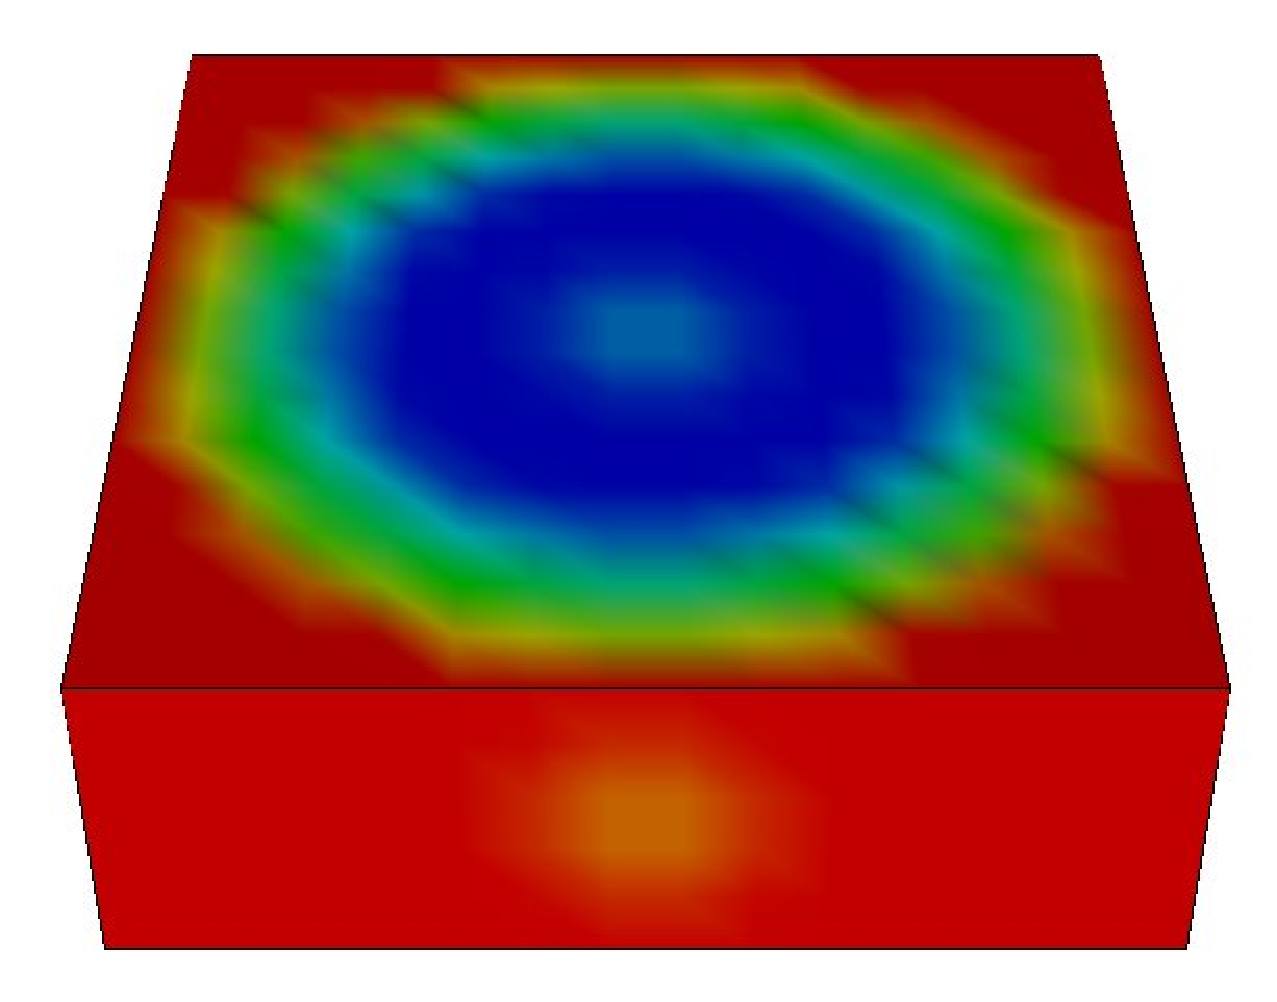
\includegraphics[width=\thumbnailwidth]{figures/Map} &
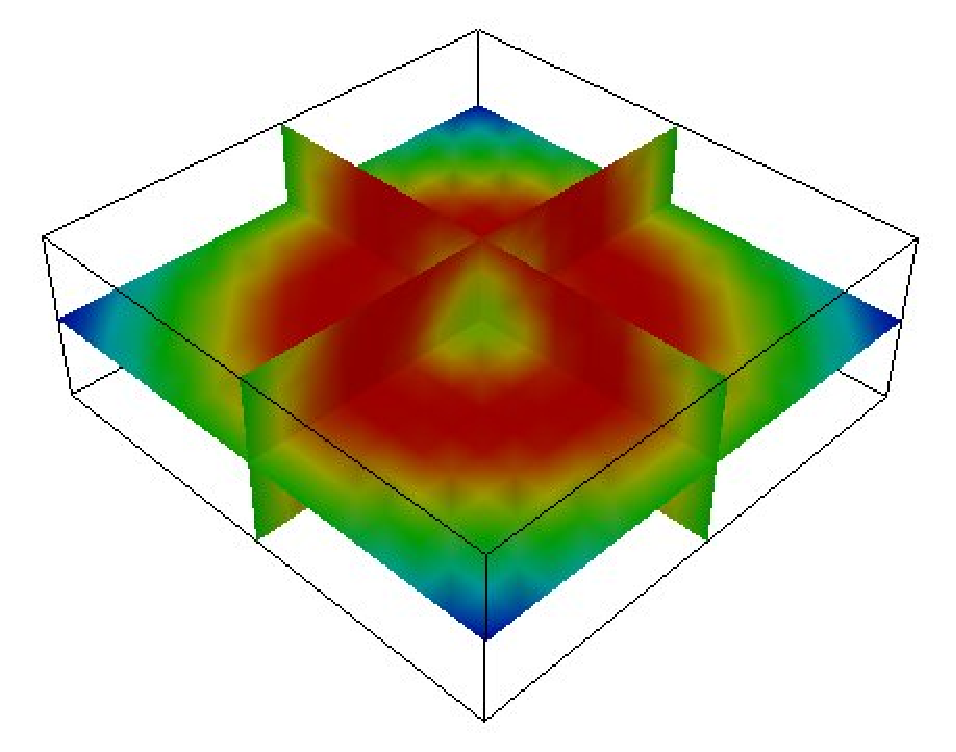
\includegraphics[width=\thumbnailwidth]{figures/MapOnPlaneCut} &
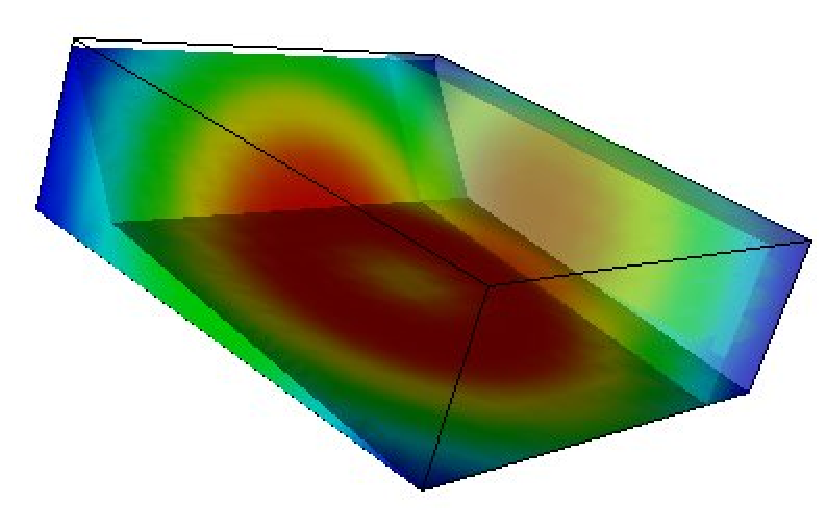
\includegraphics[width=\thumbnailwidth]{figures/MapOnPlaneClip} \\
Map & MapOnPlaneCut & MapOnPlaneClip \\
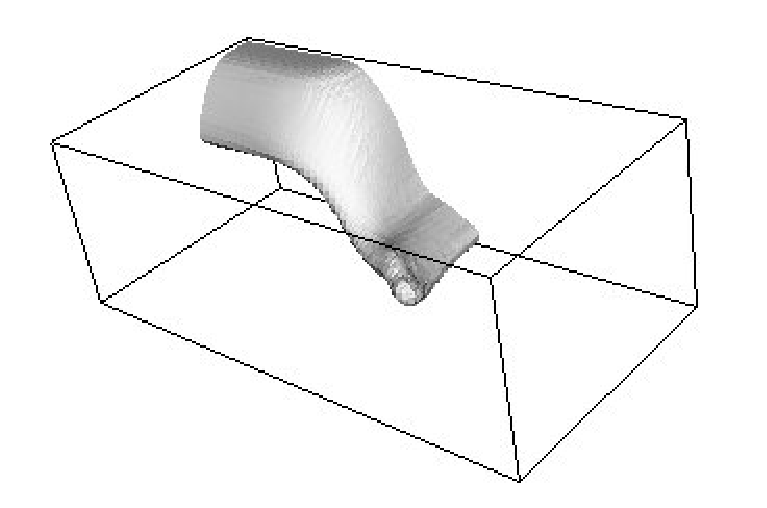
\includegraphics[width=\thumbnailwidth]{figures/MapOnScalarClip} & 
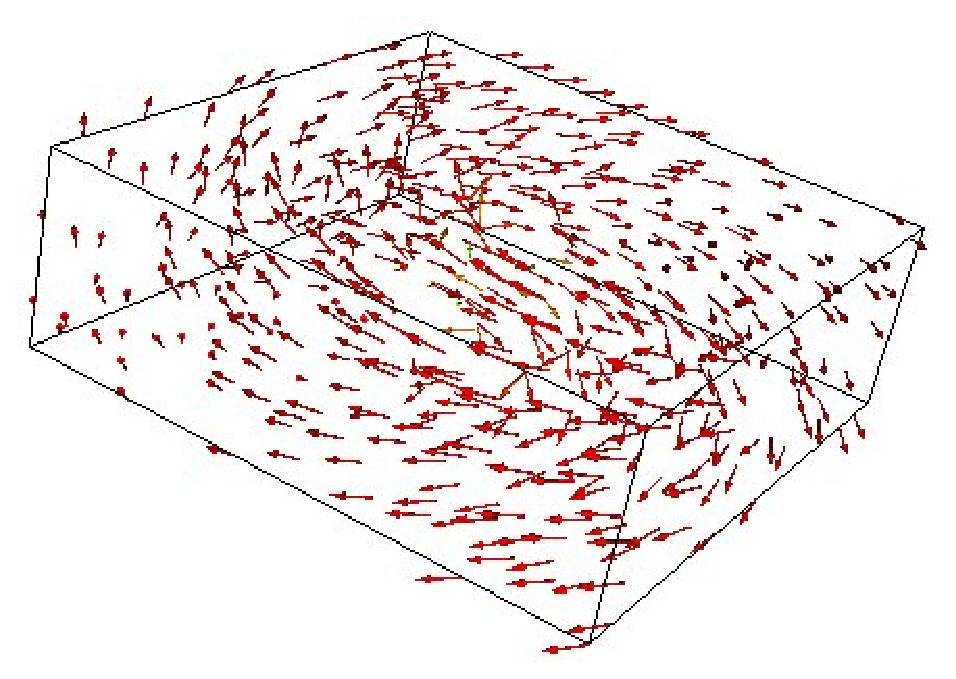
\includegraphics[width=\thumbnailwidth]{figures/Velocity} & 
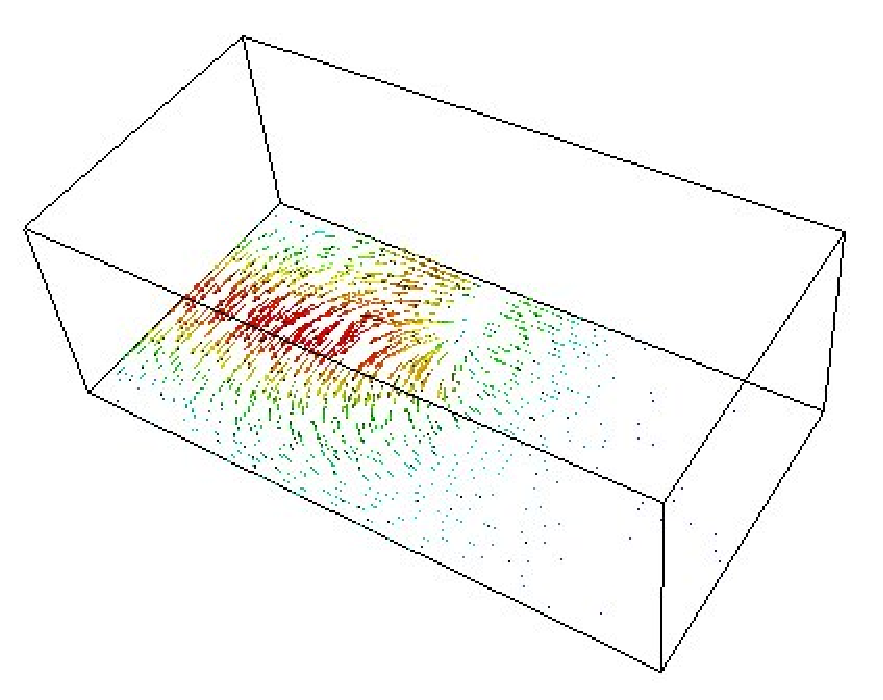
\includegraphics[width=\thumbnailwidth]{figures/VelocityOnPlaneCut}  \\
MapOnScalarClip & Velocity & VelocityOnPlaneCut \\
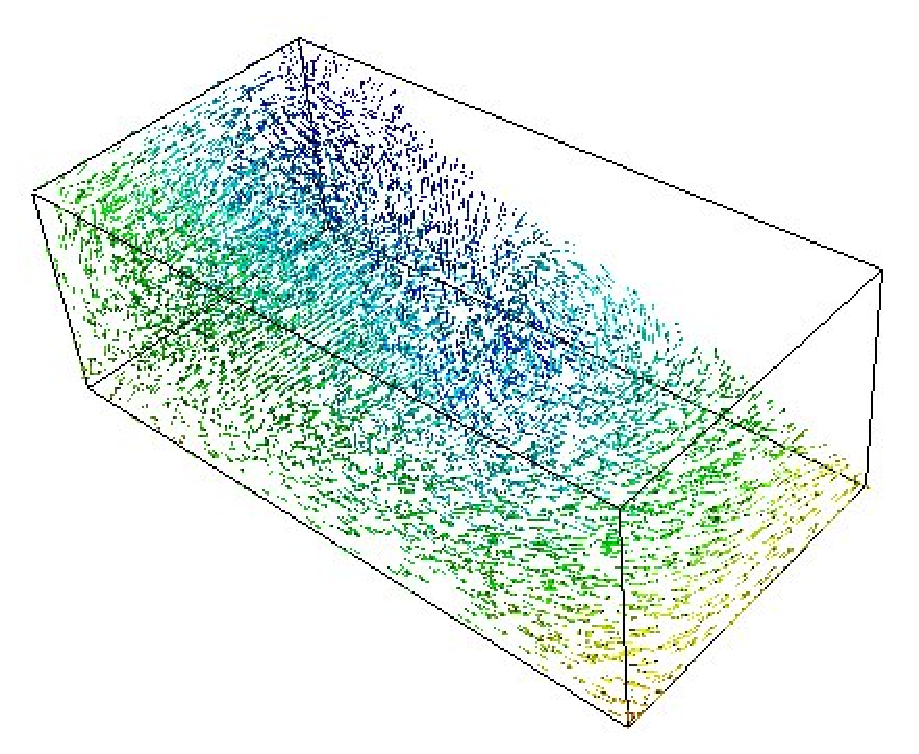
\includegraphics[width=\thumbnailwidth]{figures/VelocityOnPlaneClip} & 
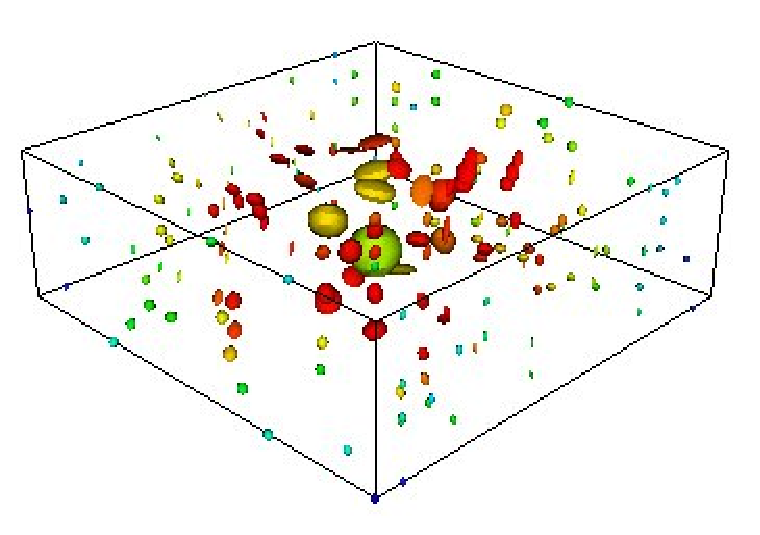
\includegraphics[width=\thumbnailwidth]{figures/Ellipsoid} & 
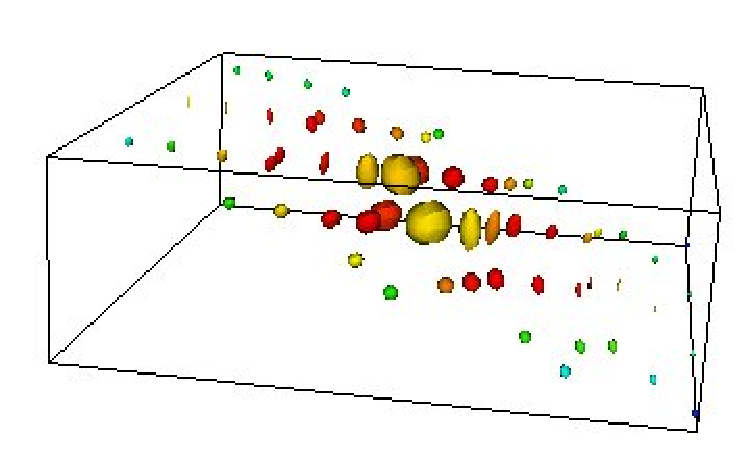
\includegraphics[width=\thumbnailwidth]{figures/EllipsoidOnPlaneCut}  \\
VelocityOnPlaneClip & Ellipsoid & EllipsoidOnPlaneCut \\
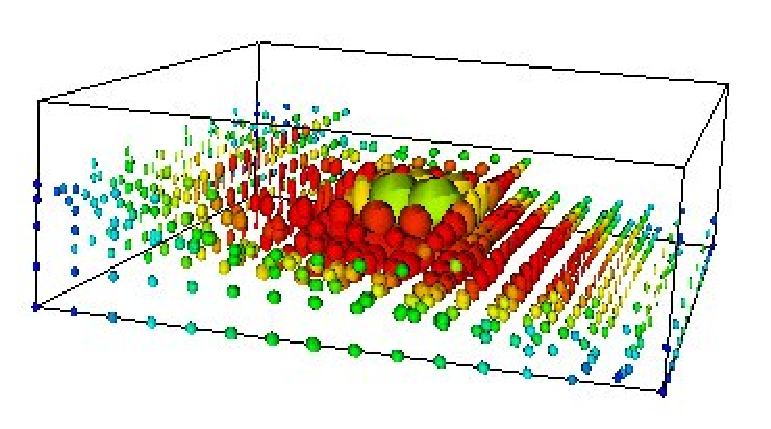
\includegraphics[width=\thumbnailwidth]{figures/EllipsoidOnPlaneClip} & 
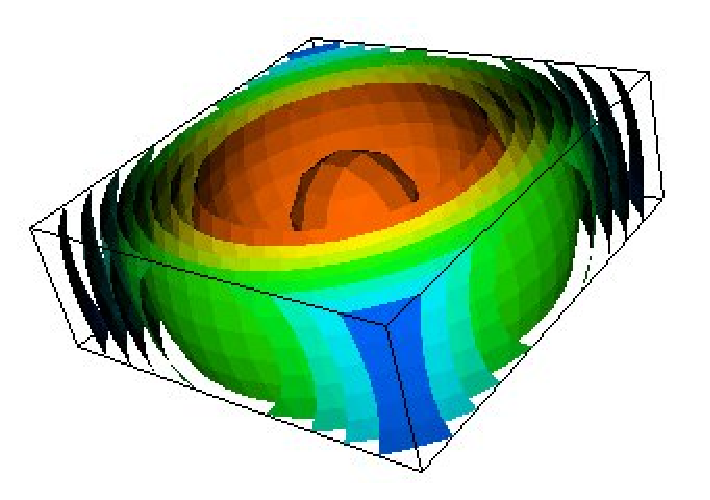
\includegraphics[width=\thumbnailwidth]{figures/Contour} & 
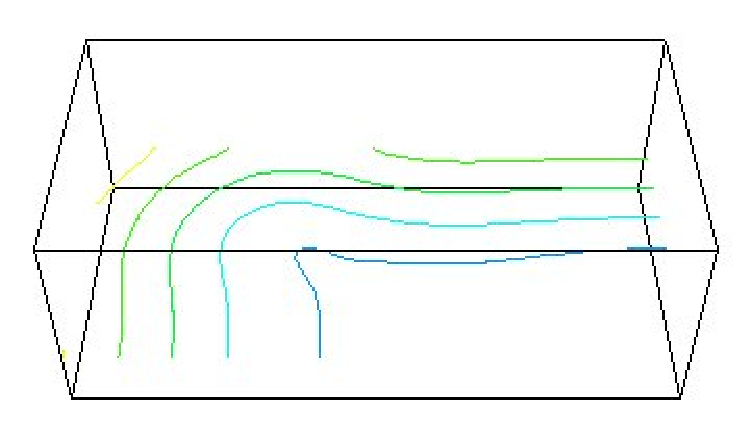
\includegraphics[width=\thumbnailwidth]{figures/ContourOnPlaneCut}  \\
EllipsoidOnPlaneClip & Contour & ContourOnPlaneCut \\
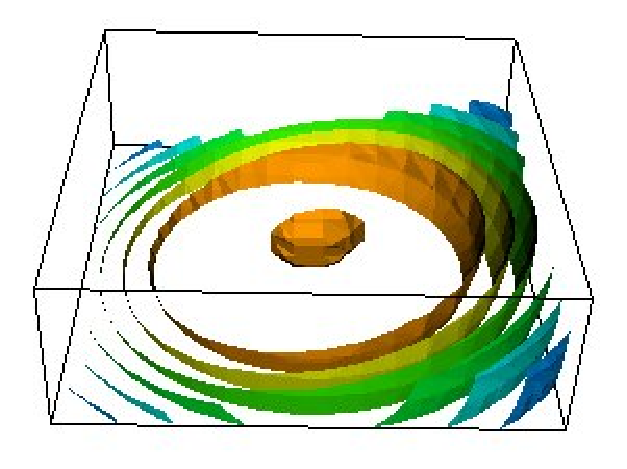
\includegraphics[width=\thumbnailwidth]{figures/ContourOnPlaneClip} & 
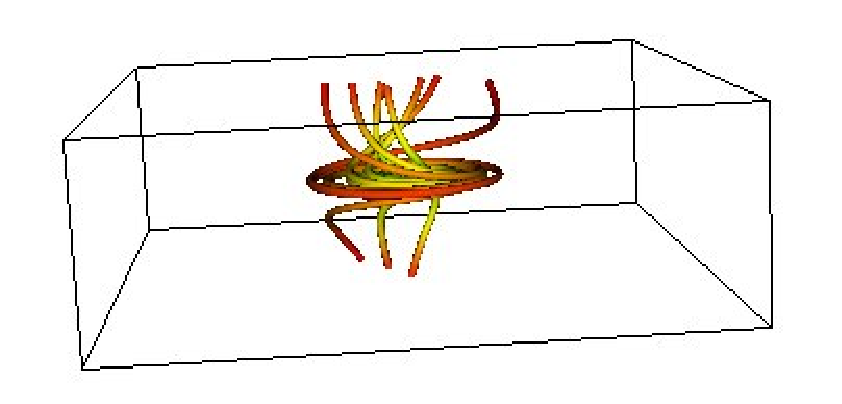
\includegraphics[width=\thumbnailwidth]{figures/StreamLine} & 
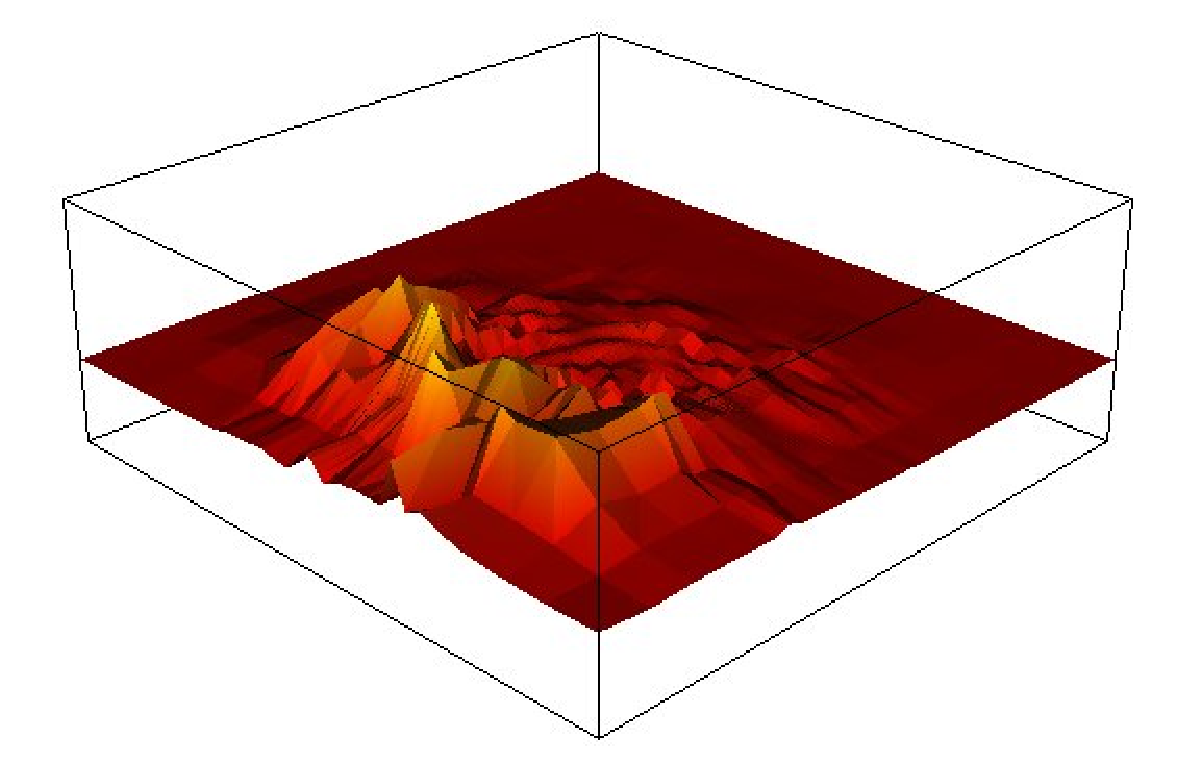
\includegraphics[width=\thumbnailwidth]{figures/Carpet}  \\
ContourOnPlaneClip & StreamLine & Carpet \\
\end{tabular}
\caption{Sample output}
\end{table}


% ############################################################################# 


\section{Complex Examples}
The following scripts show some of the more complex examples.

\textsf{Reading A Series of Files}

\begin{python}
# Import the necessary modules.
from esys.pyvisi import Scene, DataCollector, Contour, Camera 
from esys.pyvisi.constant import *

PYVISI_EXAMPLE_MESHES_PATH = "data_meshes/"
PYVISI_EXAMPLE_IMAGES_PATH = "data_sample_images/"
X_SIZE = 400
Y_SIZE = 300

SCALAR_FIELD_POINT_DATA_1 = "lava"
SCALAR_FIELD_POINT_DATA_2 = "talus"
FILE_2D = "phi_talus_lava."
FIRST_FILE_NAME = "phi_talus_lava.0099.vtu"

IMAGE_NAME = "seriesofreads"
JPG_RENDERER = Renderer.ONLINE_JPG


# Create a Scene.
s = Scene(renderer = JPG_RENDERER, num_viewport = 1, x_size = X_SIZE, 
        y_size = Y_SIZE)

# Create a DataCollector reading from a XML file. An initial file must always
# be assigned when the DataCollector is created, although the same file is 
# read again in the for-loop.   
dc1 = DataCollector(source = Source.XML)
dc1.setFileName(file_name = PYVISI_EXAMPLE_MESHES_PATH + FIRST_FILE_NAME)
dc1.setActiveScalar(scalar = SCALAR_FIELD_POINT_DATA_1)

# Create a Contour.
mosc1 = Contour(scene = s, data_collector = dc1, 
        viewport = Viewport.SOUTH_WEST, lut = Lut.COLOR, cell_to_point = False,
        outline = True)
mosc1.generateContours(0)

# Create a second DataCollector reading from the same XML file. An initial 
# file must always be assigned when the DataCollector is created, 
# although the same file is read again in the for-loop.   
dc2 = DataCollector(source = Source.XML)
dc2.setFileName(file_name = PYVISI_EXAMPLE_MESHES_PATH + FIRST_FILE_NAME)
dc2.setActiveScalar(scalar = SCALAR_FIELD_POINT_DATA_2)

# Create a second Contour.
mosc2 = Contour(scene = s, data_collector = dc2, 
        viewport = Viewport.SOUTH_WEST, lut = Lut.COLOR, cell_to_point = False,
        outline = True)
mosc2.generateContours(0)

# Read in one file one after another and render the object. 
for i in range(99, 104):
    dc1.setFileName(file_name =  PYVISI_EXAMPLE_MESHES_PATH + FILE_2D +
	        "%04d.vtu" % i)
    dc1.setActiveScalar(scalar = SCALAR_FIELD_POINT_DATA_1)
    dc2.setFileName(file_name =  PYVISI_EXAMPLE_MESHES_PATH + FILE_2D +
	        "%04d.vtu" % i)
    dc2.setActiveScalar(scalar = SCALAR_FIELD_POINT_DATA_2)

    s.render(PYVISI_EXAMPLE_IMAGES_PATH + IMAGE_NAME + "%04d.jpg" % i)
\end{python}

\textsf{Manipulating A Single File with A Series of Translation}

\begin{python}
# Import the necessary modules.
from esys.pyvisi import Scene, DataCollector, MapOnPlaneCut, Camera
from esys.pyvisi.constant import *

PYVISI_EXAMPLE_MESHES_PATH = "data_meshes/"
PYVISI_EXAMPLE_IMAGES_PATH = "data_sample_images/"
X_SIZE = 400
Y_SIZE = 400

SCALAR_FIELD_POINT_DATA = "temperature"
FILE_3D = "interior_3D.xml"
IMAGE_NAME = "seriesofcuts"
JPG_RENDERER = Renderer.ONLINE_JPG


# Create a Scene.
s = Scene(renderer = JPG_RENDERER, num_viewport = 1, x_size = X_SIZE, 
        y_size = Y_SIZE)

# Create a DataCollector reading from a XML file.
dc1 = DataCollector(source = Source.XML)
dc1.setFileName(file_name = PYVISI_EXAMPLE_MESHES_PATH + FILE_3D)
dc1.setActiveScalar(scalar = SCALAR_FIELD_POINT_DATA)

# Create a MapOnPlaneCut.
mopc1 = MapOnPlaneCut(scene = s, data_collector = dc1, 
        viewport = Viewport.SOUTH_WEST, lut = Lut.COLOR, cell_to_point = False,
        outline = True)
mopc1.setPlaneToYZ(offset = 0.1)

# Create a Camera.
c1 = Camera(scene = s, data_collector = dc1, viewport = Viewport.SOUTH_WEST)
c1.isometricView()

# Render the object with multiple cuts from a series of translation.
for i in range(0, 5):
    s.render(PYVISI_EXAMPLE_IMAGES_PATH + IMAGE_NAME + "%02d.jpg" % i)
    mopc1.translate(0.6,0,0)
\end{python}

